\documentclass[letterpaper,10pt]{article}

\usepackage{bm}
\usepackage{amsfonts}
\usepackage{amsmath}
\usepackage{graphics}




% ----------------------------------------------------------------------------------------------------------------
%Jc : Jacob comment
%Proposed, diff command for derivatives:
\newcommand{\diff}[2]{ 
\frac{\mathrm{d}#1}{\mathrm{d}#2} 
}
%Example:
% $TEST:  \diff{^2 f(x)}{x} $



% ----------------------------------------------------------------------------------------------------------------




\begin{document}

%========================================================================================
%	1D EXAMPLES
%========================================================================================
\section{1D examples}

\section{Second order differential equation}

\subsection{Producing our differential equation}

Let's produce our own differential equation so we know the exact solution. Let's try with the following polynomial

\begin{equation}
f(x) = (x-1)(x-2)(x-3) = x^3 - 6x^2 + 11x - 6
\label{eq:SecondOrderEq_SolExact}
\end{equation}

Let's get the firs two derivates

\[
\begin{array}{rl}
f'(x) = & 3x^2 - 12x + 11 \\
f''(x) = & 6x - 12x
\end{array}
\]

And our second order differential equation is

\begin{equation}
\frac{d^2 f(x)}{dx^2} = 6x - 12x
\label{eq:SecondOrderEq}
\end{equation}

This form is known as the \textbf{strong} form of the partial differential equation. Of course, later we'll have to proportionate the appropriate boundary conditions to get the function shown in \ref{eq:SecondOrderEq_SolExact}. Then let's say our problem is





\begin{equation}
\begin{array}{rl}
\displaystyle
\frac{d^2 f(x)}{dx^2} = 6x - 12x & \textrm{ in } \mathbb{R} \\ \\
\displaystyle
f(x) = 0 & \textrm{ on } x = 1 \\ \\
\displaystyle
f'(x) n_x = \frac{d f(x)}{d x} n_x = 2 & \textrm{ on } x = 3 
\end{array}
\label{eq:Problem_StrongForm}
\end{equation}


\begin{figure}
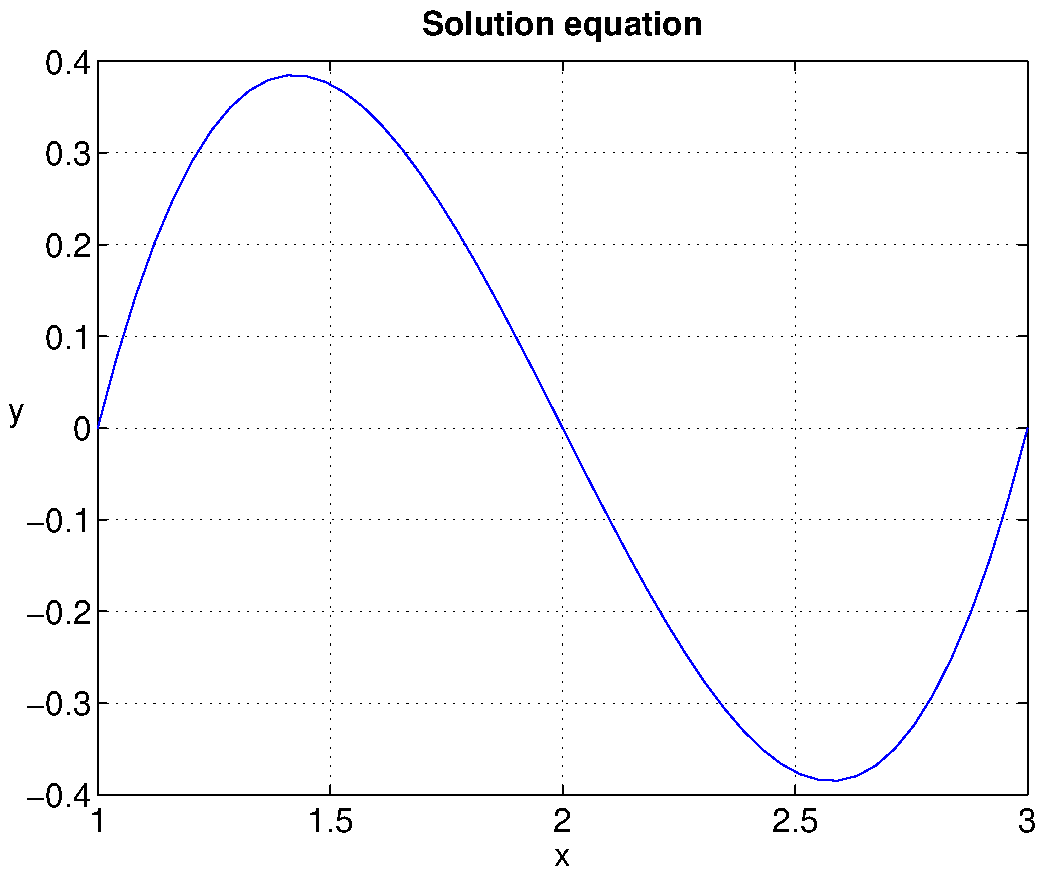
\includegraphics{figures/1_01_Objective_function.pdf}
\end{figure}



\subsection{The weak form}

In order to use the finite element method to solve this equation, the first step is to write the differential equation in the \textbf{weak} or \textbf{variational} form. To do so, we require the Green's Theorem in 1D

\[
\int_{\Omega} \frac{\partial}{\partial x} \frac{\partial u}{\partial x} \, w \, d\Omega + \int_{\Omega} \frac{\partial u}{\partial x} \frac{\partial w}{\partial x} \, d\Omega = \int_{\Gamma} \frac{\partial u}{\partial x} n_x \, w \, d\Gamma
\]

Because we'll be working in 1D, then we can use $d$ instead of $\partial$
%Jc: What does each of them mean? 



\begin{equation}
\int_{\Omega} \frac{d}{d x} \frac{d u}{d x} \, w \, d\Omega + \int_{\Omega} \frac{d u}{d x} \frac{d w}{d x} \, d\Omega = \int_{\Gamma_D} \frac{d u}{d x} n_x \, w \, d\Gamma + \int_{\Gamma_N} \frac{d u}{d x} n_x \, w \, d\Gamma
\label{eq:GreenTheorem_1D}
\end{equation}

As you can see the boundary $\Gamma$ was split into $\Gamma_D$ and $\Gamma_N$, which are the places where the \textbf{essential} (in this case Dirichlet) % Jc: maybe, "also called Dirichlet"
and \textbf{natural} (in this case Neumann) %Jc. Same here, maybe
 boundary conditions, respectively, are imposed. $w$ is known as \textbf{test function} and works as a weight to do an average version of the original (the strong form) differential equation.

Using the equations \ref{eq:GreenTheorem_1D} and \ref{eq:SecondOrderEq} and in our case $u = f(x)$

\[
\int_{\Omega} (6x-12) w \, d\Omega + \int_{\Omega} \frac{d f(x)}{d x} \frac{d w}{d x} \, d\Omega = \int_{\Gamma_D} \frac{d f(x)}{d x} n_x \, w \, d\Gamma + \int_{\Gamma_N} \frac{d f(x)}{d x} n_x \, w \, d\Gamma
\]

Reordering

\[
\int_{\Omega} \frac{d f(x)}{d x} \frac{d w}{d x} \, d\Omega + \int_{\Omega} (6x-12) w \, d\Omega - \int_{\Gamma_D} \frac{d f(x)}{d x} n_x \, w \, d\Gamma - \int_{\Gamma_N} \frac{d f(x)}{d x} n_x \, w \, d\Gamma = 0
\]

In order to impose easily the dirichlet boundary conditions we'll use a $w$ such that $w=0$ on $\Gamma_D$. So the final weak form version is

\begin{equation}
\int_{\Omega} \frac{d f(x)}{d x} \frac{d w}{d x} \, d\Omega + \int_{\Omega} (6x-12) w \, d\Omega - \int_{\Gamma_N} \frac{d f(x)}{d x} n_x \, w \, d\Gamma = 0
\end{equation}

Then the problem using the weak form would be

\begin{equation}
\begin{array}{rl}
\displaystyle
\int_{\Omega} \frac{d f(x)}{d x} \frac{d w}{d x} \, d\Omega + \int_{\Omega} (6x-12) w \, d\Omega - \int_{\Gamma_N} \frac{d f(x)}{d x} n_x \, w \, d\Gamma = 0 & \textrm{ in } \mathbb{R} \\ \\
\displaystyle
f(x) = 0 & \textrm{ on } x = 1 \\ \\
\displaystyle
f'(x) n_x = \frac{d f(x)}{d x} n_x = 2 & \textrm{ on } x = 3 
\end{array}
\label{eq:Problem_WeakForm}
\end{equation}

\subsection{Discretization and the Galerkin method}

Now its time to do the discretization part and use the famous Galerkin method. First over a finite element method the solution will be interpolated like this

\begin{equation}
f(x) \approx \sum_{i=1}^n N_i(x_i) f(x_i)
\end{equation}

The $x_i$ are the location of the nodes that define the element and $N_i(x_i)$ are the shape functions (known as \textbf{trial functions}). Because we are in 1D our elements are bars and at least we need two nodes to define it.

MISSING FIGURE

So our finite element approximation will be, if we use two nodes

\[
f(x) \approx \sum_{i=1}^2 N_i(x_i) f(x_i) = N_1(x_1) f(x_1) + N_2(x_2) f(x_2)
\]

The Galerkin method implies to use $w=N_i(x)$. Considering this and the finite element approximation over an element we get

\begin{small}
\[
\int_{\Omega^e} \frac{d f(x)}{d x} \frac{d w}{d x} \, d\Omega + \int_{\Omega^e} (6x-12) w \, d\Omega - \int_{\Gamma_N^e} \frac{d f(x)}{d x} n_x \, w \, d\Gamma = 0
\]
\begin{multline}
\int_{\Omega^e} \frac{d \left( \sum_{i=1}^2 N_i(x_i)  f(x_i) \right) }{d x} \frac{d N_i(x)}{d x} \, d\Omega + \int_{\Omega^e} (6x-12) N_i(x)\, d\Omega \\
- \int_{\Gamma_N^e} \frac{d f(x)}{d x} n_x \, N_i(x) \, d\Gamma = 0
\end{multline}
\end{small}

You may be wondering why we ketp the $f(x)$ in the last term on the left side of the equation. Well this is because this integral is for the Neumann boundary conditions as you can see in equation \ref{eq:Problem_WeakForm}. This term will be not zero only when a Neumann condition is applied on the edges of a element. From the last formulae we get a system of equations, because $i=1,2$.

\begin{multline}
\begin{bmatrix}
\displaystyle
\int_{\Omega^e} \frac{d N_1(x)}{d x} \frac{d N_1(x)}{d x} \, d\Omega &
\displaystyle
\int_{\Omega^e} \frac{d N_1(x)}{d x} \frac{d N_2(x)}{d x} \, d\Omega \vspace{2mm} \\
\displaystyle
\int_{\Omega^e} \frac{d N_2(x)}{d x} \frac{d N_1(x)}{d x} \, d\Omega &
\displaystyle
\int_{\Omega^e} \frac{d N_2(x)}{d x} \frac{d N_2(x)}{d x} \, d\Omega
\end{bmatrix}
\begin{bmatrix}
y_1 \vspace{2mm}\\
y_2
\end{bmatrix}
= \\
\begin{bmatrix}
\displaystyle
-\bar{q}_1 \int_{\Gamma_N^e} N_1(x) \, d\Gamma \vspace{2mm}\\
\displaystyle
\bar{q}_2 \int_{\Gamma_N^e} N_2(x) \, d\Gamma
\end{bmatrix}
-
\begin{bmatrix}
\displaystyle
\int_{\Gamma_N^e} (6x-12) N_1(x) \, d\Gamma \vspace{2mm}\\
\displaystyle
\int_{\Gamma_N^e} (6x-12) N_2(x) \, d\Gamma
\end{bmatrix}
\label{eq:SystemEq_Element}
\end{multline}

This is the system of equations for each element. Note we substitute $f(x_i) = y_i$ and $\frac{d f(x_i)}{d x} = \bar{q}_i$. We can take out from the integral the $f(x_i)$ because his value does not change.

Another thing is $n_x$. In this case $n_x(x_1) = -1$ and $n_x(x_2)=1$, considering $x_1 \leq x_2$. The normal's direction is taken always pointing outwards.

\subsection{The shape functions}

If you can remember we set $w=N_i(x)$ but one condition that $w$ has to respect is $w=0$ on $\Gamma_D$. Also remember the finite element approximation $f(x) \approx \sum_{i=1}^2 N_i(x_i) f(x_i)$. One way to follow this rule is make each $N_i$ take value 1 in his node and 0 on the other ones.

In this case is easy to ``guess'' the expressions for $N_1$ and $N_2$ taking in account the rule

\begin{equation}
\begin{array}{cc}
\displaystyle
N_1(x) = \frac{x_2 - x}{x_2 - x_1} & 
\displaystyle
N_2(x) = \frac{x - x_1}{x_2 - x_1}
\end{array}
\end{equation}

The next step is substitute the expressions for the shape functions in eq. \ref{eq:SystemEq_Element}

\begin{multline*}
\begin{bmatrix}
\displaystyle
\int_{x_1}^{x_2} \frac{1}{(x_2-x_1)^2} \, dx &
\displaystyle
-\int_{x_1}^{x_2} \frac{1}{(x_2-x_1)^2} \, dx \vspace{2mm} \\
\displaystyle
-\int_{x_1}^{x_2} \frac{1}{(x_2-x_1)^2} \, dx &
\displaystyle
\int_{x_1}^{x_2} \frac{1}{(x_2-x_1)^2} \, dx
\end{bmatrix}
\begin{bmatrix}
y_1 \vspace{2mm}\\
y_2
\end{bmatrix}
= \\
\begin{bmatrix}
\displaystyle
\left. -\bar{q}_1 \frac{x_2 - x}{x_2 - x_1} \right]_{x_1}^{x_2} \vspace{2mm}\\
\displaystyle
\left. \bar{q}_2 \frac{x - x_1}{x_2 - x_1} \right]_{x_1}^{x_2}
\end{bmatrix}
-
\begin{bmatrix}
\displaystyle
\left. (6x-12) \frac{x_2 - x}{x_2 - x_1} \right]_{x_1}^{x_2} \vspace{2mm}\\
\displaystyle
\left. (6x-12) \frac{x - x_1}{x_2 - x_1} \right]_{x_1}^{x_2}
\end{bmatrix}
\end{multline*}

Doing the integrals we get

\begin{equation}
\begin{bmatrix}
\displaystyle
\frac{1}{x_2-x_1} &
\displaystyle
-\frac{1}{x_2-x_1}\vspace{2mm} \\
\displaystyle
-\frac{1}{x_2-x_1} &
\displaystyle
\frac{1}{x_2-x_1}
\end{bmatrix}
\begin{bmatrix}
y_1 \vspace{2mm}\\
y_2
\end{bmatrix}
=
\begin{bmatrix}
\displaystyle
\bar{q}_1 \vspace{2mm}\\
\displaystyle
\bar{q}_2
\end{bmatrix}
-
\begin{bmatrix}
\displaystyle
-(6x_1-12) \vspace{2mm}\\
\displaystyle
6(x_2 - 12)
\end{bmatrix}
\end{equation}

\section{Bar with axial force}


\end{document}

